\documentclass[a4paper,10pt]{article}
%\documentclass[a4paper,10pt]{scrartcl}

\usepackage[utf8x]{inputenc}
\usepackage[brazil]{babel}
\usepackage{graphicx}
\usepackage{float}


\title{\textbf{Relatório do Trabalho de Simulação} \\ Avaliação e Desempenho}
\author{Professor Paulo Aguiar}
\date{2011/1}

\pdfinfo{%
  /Title    ()
  /Author   ()
  /Creator  ()
  /Producer ()
  /Subject  ()
  /Keywords ()
}

\begin{document}
\maketitle
\pagestyle{plain}
\textbf{Integrantes e suas Participações:}
\begin{itemize}
 \item Diego Fonseca Pereira de Souza   DRE:108055513
 \begin{itemize}
    \item Assinatura: \rule{6cm}{.1mm}	
    \item Participação:
    \begin{itemize}
	\item Obtenção de Resultados
	\item Confecção do Relatório
	\item Confecção dos Gráficos
	\item Teste de Validação
	\item Otimização
	\item Análise de Resultados
    \end{itemize}
 \end{itemize}
 \item Ewerton Vinicius Ramos Balthazar DRE:106044875
  \begin{itemize}
    \item Assinatura: \rule{6cm}{.1mm}	
    \item Participação:
    \begin{itemize}
	\item Obtenção de Resultados
	\item Confecção do Relatório
	\item Teste de Validação
	\item Otimização
	\item Análise de Resultados
    \end{itemize}
 \end{itemize}
 \item Gustavo Rodrigues Lima           DRE:108055416
  \begin{itemize}
    \item Assinatura: \rule{6cm}{.1mm}	
    \item Participação:
    \begin{itemize}
	\item Implementação do Simulador
	\item Depuração Do Simulador
	\item Confecção do Relatório
	\item Teste de Validação
	\item Estimativa da fase transiente
	\item Estimativa de tamanho e número de rodadas
    \end{itemize}
 \end{itemize} 
 \item Gustavo Daniel Soares Figueiredo DRE:106051068 
  \begin{itemize}
    \item Assinatura: \rule{6cm}{.1mm}	
    \item Participação:
    \begin{itemize}
	\item Implementação do Simulador
	\item Depuração Do Simulador
	\item Confecção do Relatório
	\item Teste de Validação
	\item Estimativa da fase transiente
	\item Estimativa de tamanho e número de rodadas
    \end{itemize}
 \end{itemize} 
\end{itemize}
\section{Apresentação do Problema}
   Executar uma simulação do comportamento de um sistema no qual duas filas disputam o servidor e umas das filas tem prioridade preemptiva sobre a outra.
   \begin{figure}[H]
      \center
      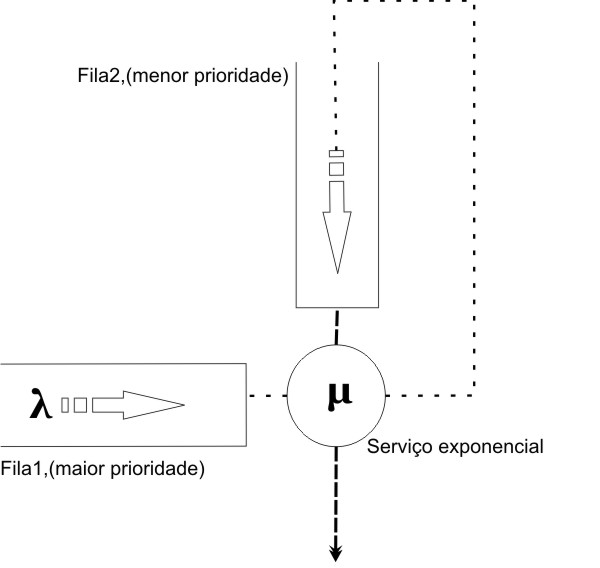
\includegraphics[scale=3]{AD-Relatorio.jpg}
      \caption{Esquema do sistema}
  \end{figure}
  Fregueses chegam à fila 1 segundo um Processo Poisson com taxa $\lambda$ (tempo entre chegadas é exponencial com taxa $\lambda$).Esta é a fila de maior prioridade do sistema.Após
  serem servidos pela primeira os fregueses seguem para a fila 2 , de menor prioridade .Ao término deste segundo serviço, os fregueses vão embora.Tanto o primeiro como o segundo 
  serviços do freguês são obtidos de forma independente a partir de uma distribuição exponencial com taxa $\mu=s^{-1}$.Isto significa que os serviços
  recebidos por um mesmo freguês são totalmente independentes.Todavia,o serviço em andamenteo da fila 2 pode ser interrompido ,pela chegada de um freguês na fila 1.Neste caso, o serviço
  interrompido será retomado de onde parou.Observe que um freguês da fila 2 poderá ser interrompido mais de uma vez.As filas operam sobre o regime \textbf{FCFS} (First Come First Servide -
  o primeiro à chegar é o primeiro à ser servido).
\section{Solução Proposta}
      \subsection{Introdução}
	\subsubsection{Funcionamento Geral do Simulador}
	\subsubsection{Os Eventos Escolhidos}
	\subsubsection{Método usado:replicativo}
	\subsubsection{Implementação do Conceito de Cores}
	\subsubsection{Escolha dos Parâmetros}
	\subsubsection{Estrutura Interna Utilizada}
	\subsubsection{Equimamentos de Teste}
	\subsubsection{Outra Informações Pertinentes}
      \subsection{Teste de Correção}
      \subsection{Estimativa da Fase Transiente}
      \subsection{Tabelas com os resultados}
      \subsection{Otimização}
      \subsection{Conclusão}
      \subsection{Anexo}
\end{document}